\documentclass[12 pt]{article}        	%sets the font to 12 pt and says this is an article (as opposed to book or other documents)
\usepackage{amsfonts, amssymb}					% packages to get the fonts, symbols used in most math
\usepackage{amsmath}
\usepackage{graphicx}\usepackage{multicol}
  
%\usepackage{setspace}               		% Together with \doublespacing below allows for doublespacing of the document

\oddsidemargin=-0.5cm                 	% These three commands create the margins required for class
\setlength{\textwidth}{6.5in}         	%
\addtolength{\voffset}{-2pt}        		%
\addtolength{\headsep}{25pt}           	%



\pagestyle{myheadings}                           	% tells LaTeX to allow you to enter information in the heading
\markright{Andrew Mayo\hfill \today \hfill}  
																									% and put the proposition number from the book
                                                	% LaTeX will put your name on the left, the date the paper 
                                                	% is generated in the middle 
                                                 	% and a page number on the right



\newcommand{\eqn}[0]{\begin{array}{rcl}}%begin an aligned equation - allows for aligning = or inequalities.  Always use with $$ $$
\newcommand{\eqnend}[0]{\end{array} }  	%end the aligned equation

%\doublespacing                         	% Together with the package setspace above allows for doublespacing of the document

\newcommand{\qed}[0]{$\square$}        	% make an unfilled square the default for ending a proof

\begin{document}												% end of preamble and beginning of text that will be printed 

\textbf{1 (c)} 

Test accuracy for CIFAR dataset: 42.08\%

\begin{figure}[h!]
  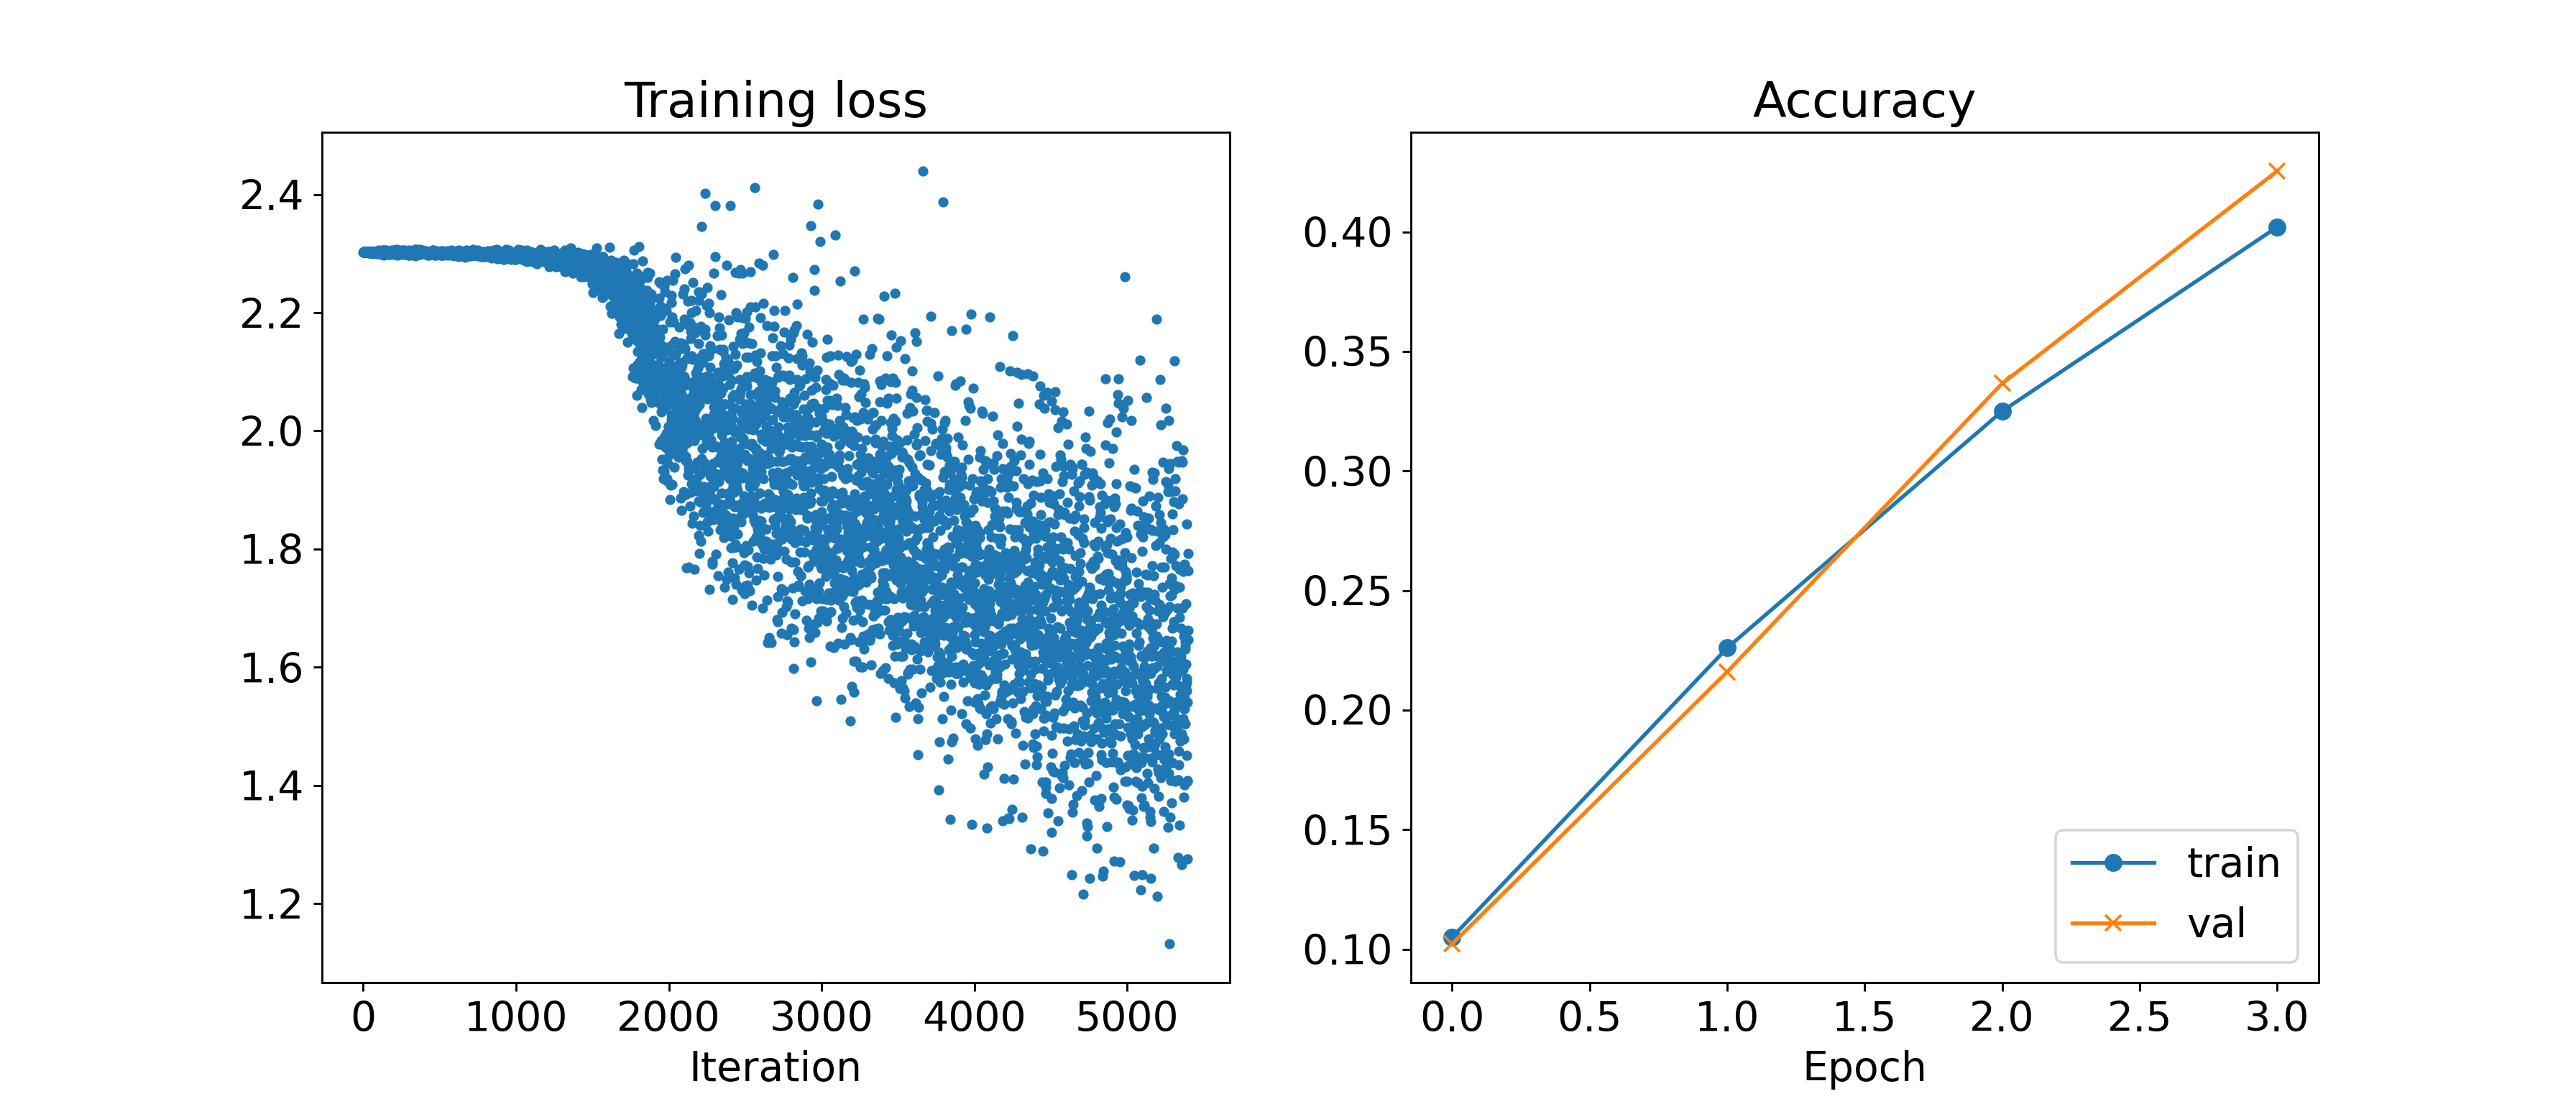
\includegraphics[width=\linewidth]{cnn.png}
\end{figure}


\textbf{2 (c)} 

\begin{figure}[h!]
  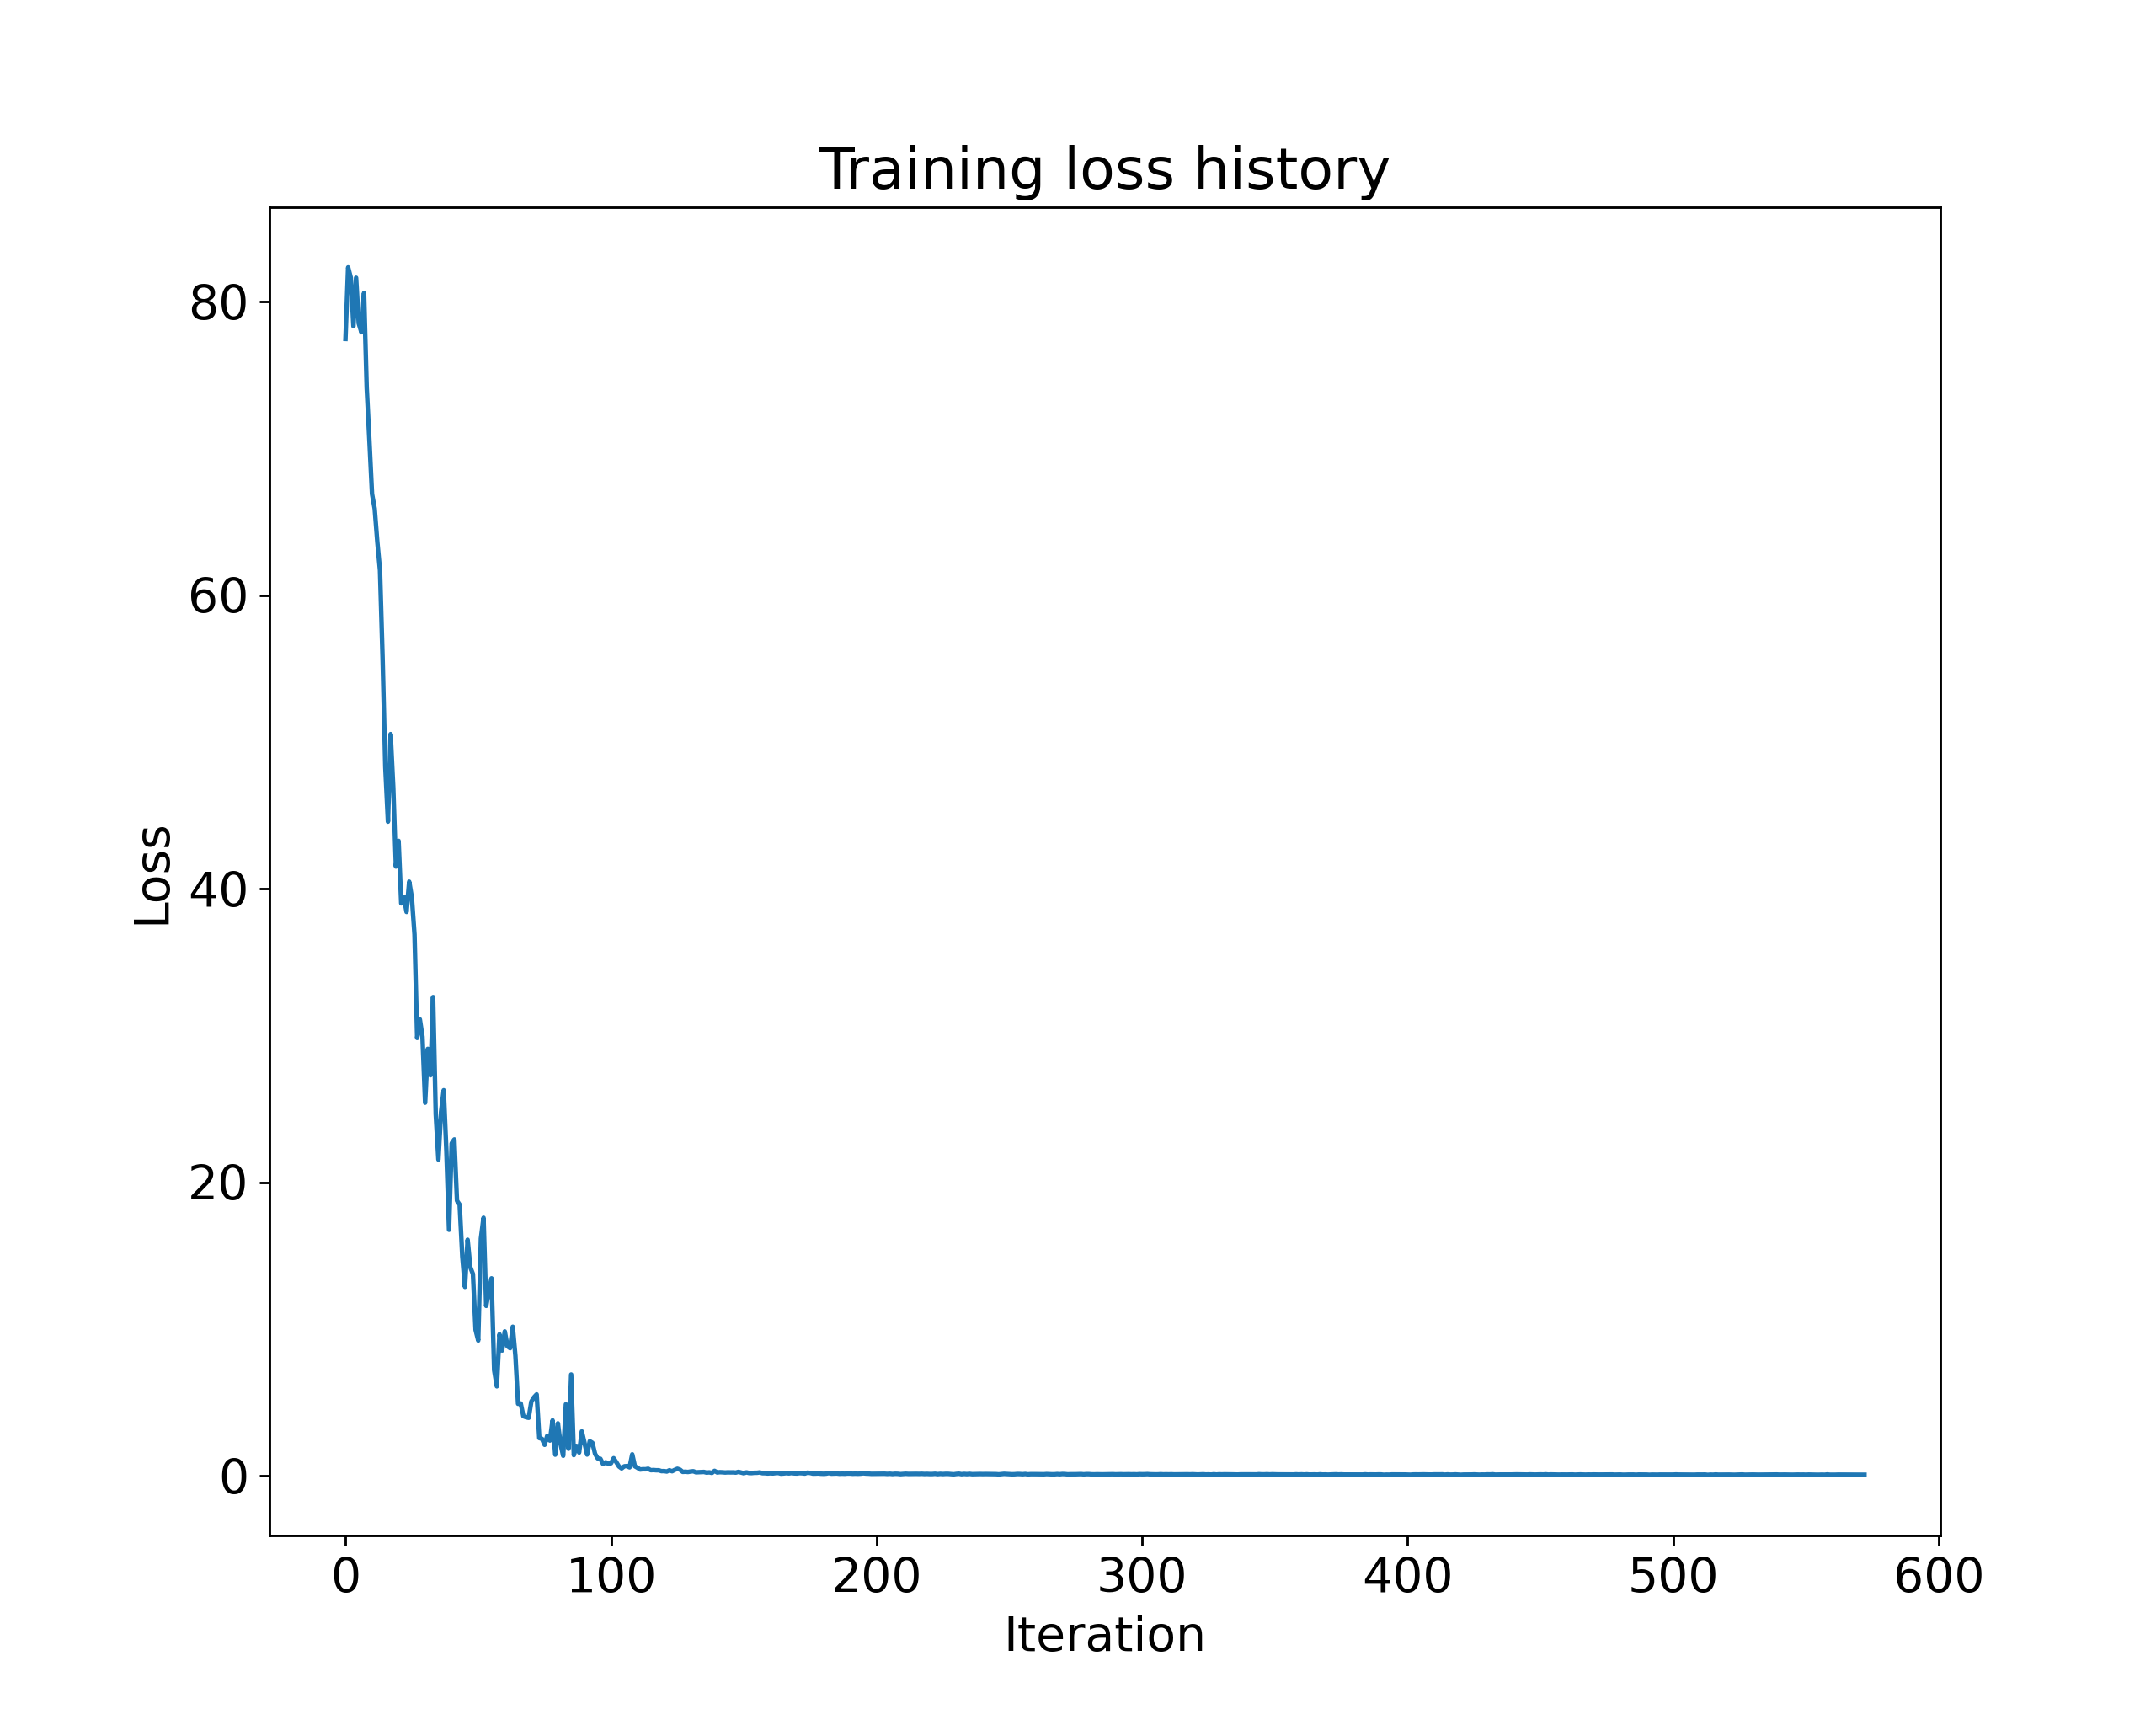
\includegraphics[width=0.5\linewidth]{image_captioning_loss.png}
\end{figure}

\begin{figure}[h!]
  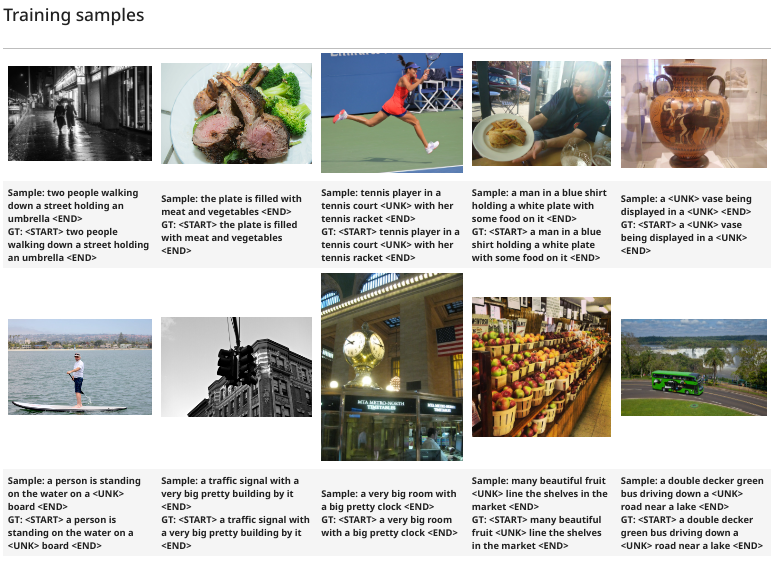
\includegraphics[width=0.7\linewidth]{captions_training.png}
\end{figure}

\begin{figure}[h!]
  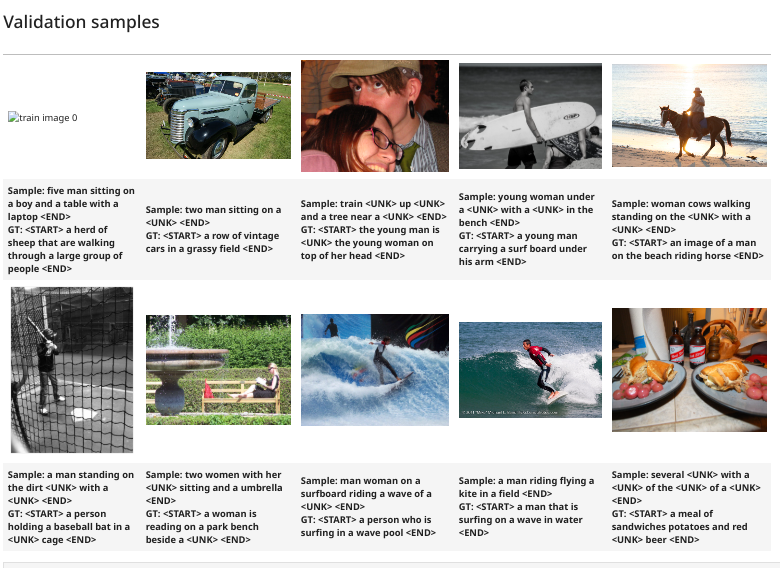
\includegraphics[width=0.7\linewidth]{captions_validation.png}
\end{figure}

\clearpage

\textbf{3 (a)}
\begin{figure}[h!]
  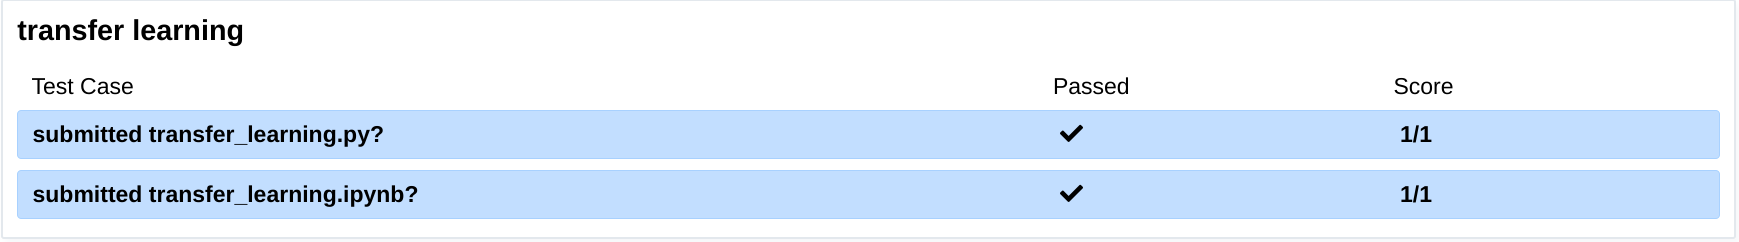
\includegraphics[width=\linewidth]{autograder_screenshot.png}
\end{figure}

\clearpage

\textbf{3 (b)}

\begin{multicols}{2}

\textbf{Fine-tuned pretrained model} \\

\begin{tabular}{ | c | c | } \hline
  Training time & 0m 0s \\
  Best val Acc & 0.712418 \\
  Epoch & 0/4 \\ \hline
        & \\
  train Loss & 0.5000 \\
  Acc & 0.7664 \\
  val Loss & 0.3085 \\
  Acc & 0.8758 \\
  Epoch & 1/4 \\ \hline
         & \\
  train Loss & 0.5936 \\
  Acc & 0.7254 \\
  val Loss & 0.2439 \\
  Acc & 0.9150 \\
  Epoch & 2/4 \\ \hline
        & \\
  train Loss & 0.5174 \\
  Acc & 0.7828 \\
  val Loss & 0.3162 \\
  Acc & 0.8824 \\
  Epoch & 3/4 \\ \hline
        & \\
  train Loss & 0.5208 \\
  Acc & 0.7705 \\
  val Loss & 0.3700 \\
  Acc & 0.8889 \\
  Epoch & 4/4 \\ \hline
        & \\
  train Loss & 0.7435 \\
  Acc & 0.7910 \\
  val Loss & 0.3417 \\
  Acc & 0.8562 \\
  Training time & 0m 6s \\
  Best val Acc & 0.915033 \\ \hline
\end{tabular}

\textbf{Frozen model} \\

\begin{tabular}{ | c | c | } \hline
  Training time & 0m 0s \\
  Best val Acc & 0.457516 \\
  Epoch & 0/4 \\ \hline
        & \\
  train Loss & 0.5814 \\
  Acc & 0.7049 \\
  val Loss & 0.2089 \\
  Acc & 0.9346 \\
  Epoch & 1/4 \\ \hline
        & \\
  train Loss & 0.4798 \\
  Acc & 0.7910 \\
  val Loss & 0.1932 \\ 
  Acc & 0.9477 \\
  Epoch & 2/4 \\ \hline
        & \\
  train Loss & 0.5531 \\
  Acc & 0.7336 \\
  val Loss & 0.6048 \\
  Acc & 0.7647 \\
  Epoch & 3/4 \\ \hline
        & \\
  train Loss & 0.6411 \\
  Acc & 0.7418 \\
  val Loss & 0.1941 \\
  Acc & 0.9346 \\
  Epoch & 4/4 \\ \hline
        & \\
  train Loss & 0.4340 \\
  Acc & 0.8197 \\
  val Loss & 0.2179 \\
  Acc & 0.9281 \\
  Training time & 0m 4s \\
  Best val Acc & 0.947712 \\ \hline
\end{tabular}

\end{multicols}

\newpage

\textbf{3 (c)}

\begin{figure}[h!]
  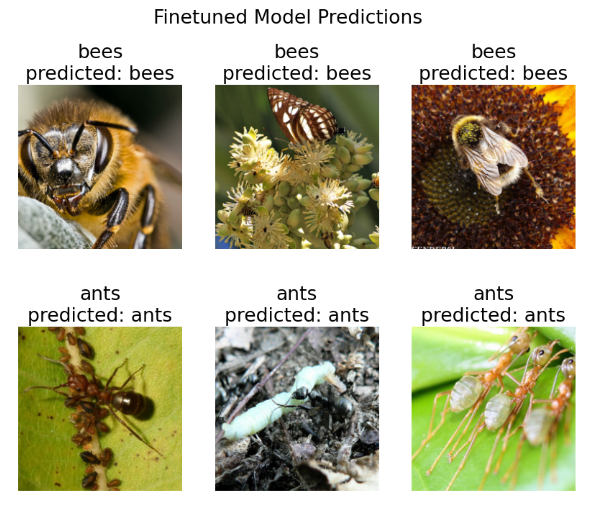
\includegraphics[width=0.6\linewidth]{tl_finetuned.png}
\end{figure}

\begin{figure}[h!]
  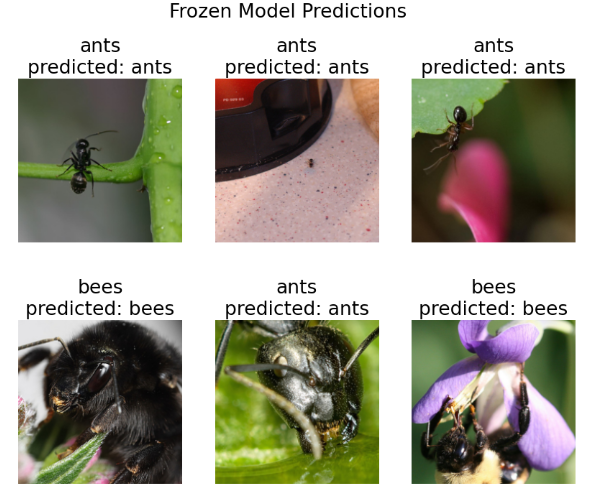
\includegraphics[width=0.6\linewidth]{tl_frozen.png}
\end{figure}

\clearpage

\textbf{4 (b)} train accuracy: 98.97\% test accuracy: 91.35\%

\textbf{4 (c)}
Iteration 15000/15000: training loss 0.6052

Story (1): 
Once upon a time, there was a little girl named Lily. She loved to read books with pretty paint. One day, while she was reading, she noticed a big book. It said, "It is ready to try me!" Lily showed her friend, telling her a welk on the book and turned it into small pillow.
"Can I have some fun for your toys, Lily?" she asked.
"Yes, you can, Lily," the well replied.
"Sure, little girl," said the well. "You can have fun at the book with your friends."
The well bookes and listens. Lily felt happy and sad turns to have a nice toy. But she loves how to make dangerous foocers when it's flexible and starts patiently, but it is big. She closes the door and seees many danger. She feels sad and cries. She cries, "I will tell you her. I will not be found my string now. But that's how you make up noise." Her mom hugs her and says, "You are silly, little girl. You are meals." The girl says, "You are tooo many. Lily and her mist is very sorrry. Thank you, mom. You are my friend." Anna says, "I love you. I love you tooo!"

Story (2): 
Once there was an old little dog named Max. Max wanted to play with his toys in the bathroom, so Max could run and play with his toys and run around in the park. But Max saw a toy car with a badge ring he could not help. His owner had a big, big, wet fountain, but Max could not find it," Max said.
Mix was sad, but he was afraid he could not do it again. He did not want to lose the toy, but he was very disappointed. He wanted to help Max. Lucy tools to help Max frint his toy but he did not work if he would help him find it.
"Max, help me feel bettter!" Lucy said. She gove the toy but it was dark. She felt a bit bit sorrry. She wanted a block by the house, but no one helped him.
"I'm sorrry, mister. I did not mean to stay rude. I know a generous bird with you. I love you." Lucy asked.
"I will help you, help me find your own stick. I love you tooo. But you have to learn to be kind. Thank you, dad think for matching me gett here. When I learn you," Lucy and Ben said.
They went back to play with their blocks. They loved the blue st

Story (3): 
One day, she could wait for her mom to close her eyes to her. She saw a toy car filled with marks on it. The toy was broken and shiny.
Sunday, Snowy noticed that Lily was scared on her mom's toy car. She looked at Tom and saw Lily's mark on the cape. Together, they found a box on a high cape. They decided to touch it and talk to the duck. Finally, they found Lily's cape. Lily felt bad for touching the patch. "It's not nice," she said. "You can seee your mark and build the house," Lily said. She laughed and said, "Okay, we can find a bucket to this whole patch for you."
At the patch, Lily saw the patch with how to find the patch. She had an idea. She took a smalll hat and toook a big bite. She stoood up and wrapped the patch on the flooor she ran acrosss the patch of the patch with her thole. She smiled and said, "Look, Lily, I am a man playing with your thoughts! Can I help your hand when you clean your rooom with a sweep to share them with your friends? That was time to be friends." Lily and Ben felt bettter and th


\end{document}
